% day1_seg1_heuristic/runavg.tex
\begin{frame}
  \onslide<1->{\frametitle{Simple Example:  Running Averages}}
 \begin{itemize}
  \onslide<2->{ \item Suppose we want to estimate some quantity like the
 resistance of a single resistor.  We have ...}
\begin{itemize}
  \onslide<3->{ \item a voltmeter with which to make measurements}
  \onslide<4->{ \item a model for the resistance: the "true" value $x$ of the resistance is assumed to be
constant in time: $x(k+1) = x(k)$}
\end{itemize}
  \onslide<5->{ \item We wish to take repeated measurements $z$ of the resistance using the voltmeter}
  \onslide<6->{ $z(1), z(2), \ldots$}
\end{itemize}
\end{frame}

\begin{frame}
  \onslide<1->{\frametitle{Simple Example: Running Averages}}
\begin{itemize}
  \onslide<2->{\item The \textbf{\textit{state}} that we are trying to estimate is the resistance of the resistor}
  \onslide<3->{\item We don't know what the state is.  (Otherwise, we wouldn't need to take measurements)}
  \onslide<4->{\item Our \textbf{\textit{state dynamics}}  or \textbf{\textit{process model}} is very simple:  The state is 1-dimensional and does not change with time:
\[x(k+1) = x(k)\]}
\end{itemize} 
\end{frame}

\begin{frame}
  \onslide<1->{\frametitle{Simple Example: Running Averages}}
\begin{itemize}
  \onslide<2->{\item What is the best way to estimate the state of our system?}
  \onslide<3->{\item In the absence of any other information, we should probably just average the measurements}
  \onslide<4->{\item We assume that the averages are unbiased, i.e., the measurement errors have zero mean}
\end{itemize} 
\end{frame}

\begin{frame}
  \onslide<1->{\frametitle{Simple Example:  Running Averages}}
 \begin{itemize}
  \onslide<2->{ \item Simple running average is like a Kalman filter with
 trivial dynamics ($x(k+1)=x(k)$)}
\end{itemize}
  \onslide<3->{Given a sequence of random measurements,$z(1),z(2),\ldots$, compute at each stage 
the best estimate of the true value of the state:  At the $n+1^{\text{st}}$
step, your best guess would be the average of all previous values:}
  \onslide<4->{\begin{equation}\label{runavg}
\hat{x}(k+1)=\dfrac{1}{k}\sum_{j=1}^{k}z(j)=\dfrac{1}{k}[\;z(1)+z(2)+\cdots+z(k)\;]
\end{equation}}
\end{frame}

\begin{frame}
 \onslide<1->{\frametitle{Simple Example:  Running Averages}}
 \begin{itemize}
 \onslide<2->{\item Q: Why is the average of all previous measurements the "best" estimate?}
 \onslide<3->{\item A: The dynamics tell us that the quantity to be estimated is not changing, and
the only variability stems from the measurements, i.e., the measurement noise}
 \onslide<4->{\item Hence, we should try to eliminate the measurement variability by averaging the measurements}
\end{itemize}
\end{frame}

\begin{frame}
\onslide<1->{\frametitle{Recursive Running Average}}
\begin{itemize}
 \onslide<2->{ \item Therefore, as much as possible, we want to rid ourselves of the noise by averaging}
 \onslide<3->{ \item Assume that noise is zero-mean, i.e., its average tends to zero over the long run}
 \onslide<4->{ \item If we had a bias, we wouldn't call that noise; that would be a systematic error on the part of our voltmeter.  We'd have to calibrate it out.}
  \onslide<5->{\item Noise can't be calibrated out; we have to average it out over time}
\end{itemize}
\end{frame}

\begin{frame}
\onslide<1->{\frametitle{Recursive Running Average}}
\onslide<2->{\begin{figure}
%\input{day1_seg1_heuristic/resistor.latex}
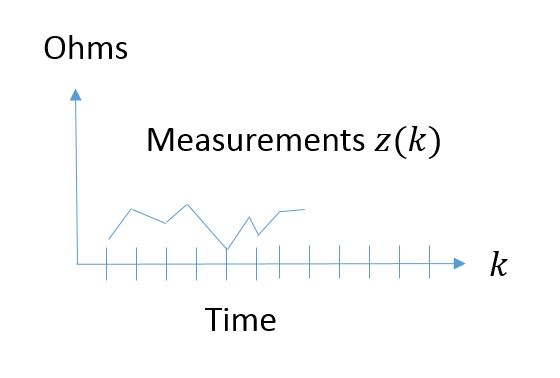
\includegraphics[width=0.75\textwidth]{day1_seg1_heuristic/resistor.jpg}
\end{figure}}
\end{frame}

\begin{frame}
\onslide<1->{\frametitle{Recursive Running Average}}
\onslide<2->{(Eq.\eqref{runavg})\\
\[\hat{x}(k+1)=\dfrac{1}{k}\sum_{j=1}^{k}z(j)=\dfrac{1}{k}[\;z(1)+z(2)+\cdots+z(k)\;]\]}
\begin{itemize}
\onslide<3->{ \item Now suppose our estimating task is going to continue for a long time and we don't want to fill up our
computer memory with a record of all the measurements taken since the start}
\onslide<4->{ \item We just want to use the previously calculated value and add a small adjustment}
\end{itemize}
\end{frame}

\begin{frame}
\onslide<1->{Step-by-Step Derivation:}
{\small \begin{align*}
  \onslide<2->{\hat{x}(k+1) &=\dfrac{1}{k}\sum_{j=1}^{k}z(j) \text{\;\;\;\;\;\;\;\;\;\;\;\;\;\;\;\;\;\;\;\;\;\;by def. Eq. }\eqref{runavg}\\}
  \onslide<3->{&=\dfrac{1}{k}\sum_{j=1}^{k-1}z(j)+\dfrac{1}{k}z(k)  \text{\;\;\;\;\;\;separate last term from sum} \\}
  \onslide<4->{&=\dfrac{1}{k}\cdot\dfrac{k-1}{k-1}\sum_{j=1}^{k-1}z(j)+\dfrac{1}{k}z(k) \text{\;\;\;\;\; multiply by 1 }\\}
  \onslide<5->{&=\dfrac{k-1}{k}\cdot\dfrac{1}{k-1}\sum_{j=1}^{k-1}z(j)+\dfrac{1}{k}z(k) \text{\;\;\; rearrange }\\}
  \onslide<6->{&=\dfrac{k-1}{k}\hat{x}(k)+\dfrac{1}{k}z(k) \text{\;\;\;\;\;\;\;\;\;\;\;\; by def. Eq. }\eqref{runavg}\text{ again}\\}
  \onslide<7->{&=\hat{x}(k) -\dfrac{1}{k}\hat{x}(k) +\dfrac{1}{k}z(k)\text{\;\;\;\;\;\;\; distribute and simplify }\\}
  \onslide<8->{&=\hat{x}(k)+\dfrac{1}{k}\left[\;z(k)-\hat{x}(k)\;\right]. \text{\;\;\;\;\;\; rearrange and factor out 1/$k$ }}
\end{align*}
}
\end{frame}

\begin{frame}
\onslide<1->{\frametitle{\textit{\textbf{Recursive}} Running Average}}
 \begin{itemize}
   \onslide<2->{\item We now have a recursive algorithm for computing a running average}
 \begin{itemize}
 \onslide<3->{\item Recipe: Take new measurement, subtract off old average and weight
 the resulting residual by a gain of $1/k$}
 \onslide<4->{\item Add this weighted residual to the old average and, voil\`{a},
 you have the new average!}
 \end{itemize}
\end{itemize}
\end{frame}

\begin{frame}
\onslide<1->{\frametitle{Recursive Running Average}}
 \begin{itemize}
 \onslide<2->{\item Note that you do not have to remember all the previous
 values or averages, only the last average}
 \onslide<3->{ \item Note also that as $k$ goes to $\infty$, the gain $1/k$ goes
 to 0. (The filter is going to sleep!)}
\end{itemize}
\onslide<4->{\begin{equation}\label{recursiverunavg}
\hat{x}(k+1)=\hat{x}(k)+\dfrac{1}{k}\left[z(k)-\hat{x}(k)\right]
\end{equation} 
}
\end{frame}

\begin{frame}
\onslide<1->{\frametitle{Recursive Running Average}}
 \begin{itemize}
  \onslide<2->{\item The residual $z(k)-\hat{x}(k)$ is the difference between the actual new measurement and what we expected or predicted the new measurement to be}
  \onslide<3->{\item Why is $\hat{x}(k)$ our predicted measurement?}
  \onslide<4->{\item Answer: In the absence of new information, the previous estimate is the only thing we have to go on!}
 \end{itemize}
\end{frame}

\begin{frame}
\onslide<1->{\frametitle{Recursive Running Average\\
MATLAB Scripts: runavgdemo.m, recursive\_avg.m}}
% \begin{itemize}
%  \item See Matlab scripts % \begin{verbatim}recursive_avg.m, static_state.m\end{verbatim}
% \end{itemize}
\onslide<2->{
\begin{figure}
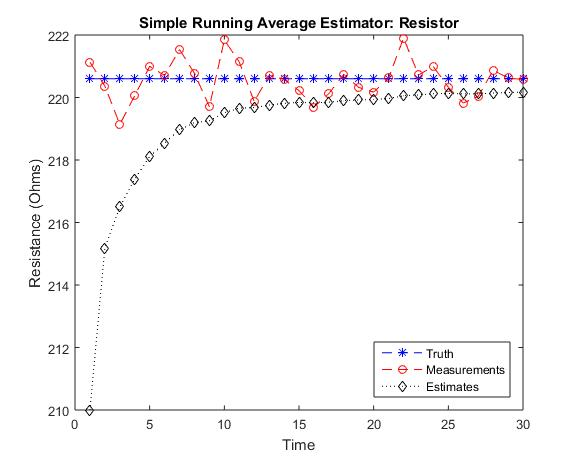
\includegraphics[width=0.75\textwidth]{day1_seg1_heuristic/runavgplot.jpg}
\end{figure}
}
\end{frame}

